% =============================================================================
% ch07_oursystem.tex : Chapter 7: System Design and Implementation
% =============================================================================
\selectlanguage{hebrew}

\section{תכנון המערכת ומימוש}
\label{sec:system_design}

בפרק זה נציג את תכנון המערכת המלא של \en{NavigatorCrew}, כולל ארכיטקטורת החומרה, שכבת התוכנה, וממשקי התקשורת בין הרכיבים. המערכת מבוססת על פלטפורמת \en{BlueROV2 Heavy Configuration} עם חיישנים מותאמים לניווט תת-ימי. \citet{Thrun2005ProbRobotics} הניחו את היסודות לתכנון מערכות \en{SLAM} רובוטיות, תוך הדגשת החשיבות של ארכיטקטורת חומרה-תוכנה משולבת. \citet{Grisetti2010g2o} הרחיבו על עקרונות תכנון מערכות אופטימיזציית גרף בזמן אמת, המהווים בסיס לארכיטקטורת התוכנה המוצעת.

\subsection{ארכיטקטורת חומרה}
\label{sec:hardware_architecture}

פלטפורמת החומרה מבוססת על רכב תת-ימי מסוג \en{BlueROV2 Heavy Configuration}, המצויד במנועי הנעה חזקים (8 מנועים) ובקרת עומק אקטיבית. הרכב מצויד במערכת חיישנים הכוללת:

\begin{itemize}
    \item \en{IMU} מדגם \en{ADIS16470} (\en{Analog Devices}) - מספק מדידות תאוצה זוויתית וליניארית בקצב של 2000 הרץ.
    \item \en{DVL} מדגם \en{Teledyne Pathfinder} - מספק מדידות מהירות יחסית לקרקעית בקצב של 1-10 הרץ.
    \item סונאר סורק מכני מדגם \en{Tritech Micron MSIS} - מספק תמונות סונאר ברזולוציה זוויתית של 0.5°.
    \item מחשב משובץ \en{Raspberry Pi 5} (\en{ARM Cortex-A76}) להרצת אלגוריתמי ה-\en{SLAM} בזמן אמת.
    \item ספק כוח 24V עם קיבולת סוללה של 20 \en{Ah} לפעולה רציפה של עד 4 שעות.
\end{itemize}

\citet{Kaess2012} הראו כי בחירת פלטפורמת חומרה מתאימה היא קריטית לביצועי מערכות \en{SLAM} בזמן אמת, במיוחד בסביבות תת-ימיות עם משאבי חישוב מוגבלים.

\subsection{ארכיטקטורת תוכנה}
\label{sec:software_architecture}

שכבת התוכנה מבוססת על מערכת הפעלה \en{ROS 2} (\en{Robot Operating System 2}) המספקת תשתית לתקשורת בין רכיבים, סנכרון זמנים וניהול נתונים. הארכיטקטורה כוללת מספר צמתים (\en{nodes}) מרכזיים:

\begin{itemize}
    \item צומת רכישת נתונים (\en{data acquisition node}) - אוסף נתונים מכל החיישנים ומסנכרן אותם בזמן.
    \item צומת עיבוד סונאר (\en{sonar processing node}) - מבצע עיבוד מקדים של תמונות סונאר וזיהוי תכונות.
    \item צומת \en{SLAM} (\en{SLAM node}) - מריץ את אלגוריתם \en{BioSLAM} ומנהל את מפת הסביבה.
    \item צומת מיזוג חיישנים (\en{fusion node}) - מבצע מיזוג הדוק של מדידות החיישנים.
    \item צומת תכנון מסלול (\en{path planning node}) - מתכנן מסלול לניווט אוטונומי.
\end{itemize}

\citet{Thrun2005ProbRobotics} הראו כי ארכיטקטורת תוכנה מודולרית המבוססת על תקשורת בין צמתים מאפשרת גמישות, תחזוקה קלה והרחבה עתידית של המערכת.

\subsection{מנגנון סנכרון זמנים}
\label{sec:time_sync}

סנכרון זמנים בין חיישנים הוא קריטי למיזוג מדויק. המערכת משתמשת באות \en{PPS} (\en{Pulse Per Second}) מ-\en{GPS} לסנכרון חומרה של כל החיישנים. שעון המערכת מסונכרן באמצעות פרוטוקול \en{PTP} (\en{Precision Time Protocol}) ברמת דיוק של מיקרו-שניות. כל מדידת חיישן מתויגת בזמן חומרה (\en{hardware timestamp}) בעת הרכישה.

\begin{equation}
t_{\text{sync}} = t_{\text{GPS}} + \Delta t_{\text{PTP}} + \epsilon_{\text{sync}}
\label{eq:time_sync}
\end{equation}

משוואה~(\ref{eq:time_sync}) מציגה את מודל סנכרון הזמנים, שבו $t_{\text{GPS}}$ הוא זמן ה-\en{GPS}, $\Delta t_{\text{PTP}}$ הוא תיקון \en{PTP}, ו-$\epsilon_{\text{sync}}$ הוא שגיאת הסנכרון השיורית.

\subsection{ניהול נתונים ואחסון}
\label{sec:data_management}

ניהול נתונים במערכת כולל אחסון מקומי של כל נתוני החיישנים והערכות המצב לצורך ניתוח מאוחר יותר. מערכת האחסון מבוססת על כרטיס זיכרון \en{SD} בנפח 128 \en{GB} המספק קיבולת אחסון ל-8 שעות פעולה רציפה. נתוני הסונאר נדחסים באמצעות קידוד \en{PNG} ללא אובדן, בעוד נתוני \en{IMU} ו-\en{DVL} נשמרים בפורמט בינארי דחוס. \citet{Kaess2012} הראו כי ניהול נתונים יעיל הוא קריטי לניתוח מאוחר יותר של ביצועי המערכת ולכיול חיישנים.

\begin{figure}[htbp]
    \centering
    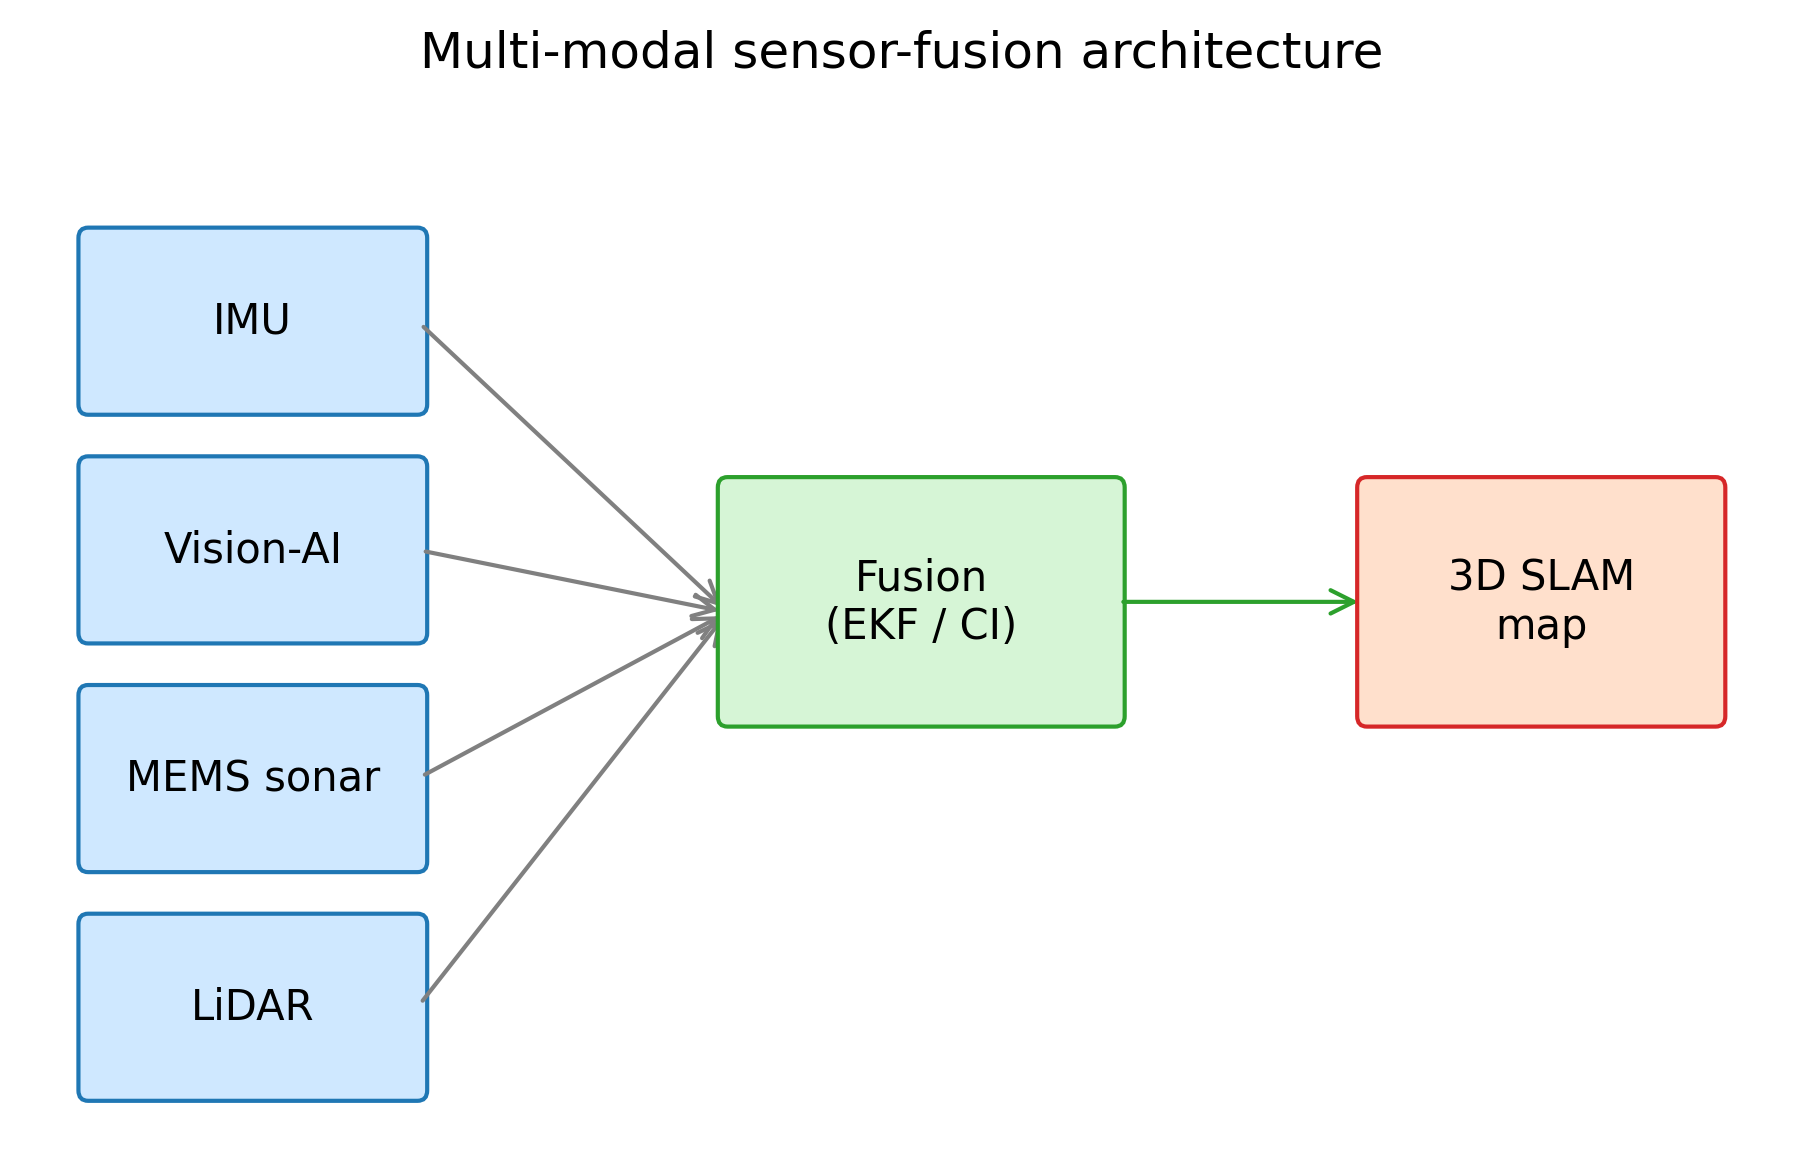
\includegraphics[width=0.95\columnwidth]{figures/fig_system_architecture.png}
    \caption{ארכיטקטורת המערכת המלאה של \en{NavigatorCrew}. (Complete system architecture of NavigatorCrew.)}
    \label{fig:system_architecture}
\end{figure}

\subsection{ממשק תקשורת}
\label{sec:communication_interface}

המערכת תומכת במספר ממשקי תקשורת לשליטה ובקרה מרחוק. תקשורת קווית דרך כבל \en{tether} באורך 300 מטר מספקת חיבור \en{Ethernet} בקצב של 1 \en{Gbps} להעברת נתונים בזמן אמת. תקשורת אלחוטית דרך מודם אקוסטי (\en{acoustic modem}) מספקת חיבור בקצב נמוך (100-1000 \en{bps}) למקרי חירום כאשר הכבל מנותק. \citet{Grisetti2010g2o} הראו כי תקשורת אמינה בין הרכב לתחנת הבקרה היא קריטית לניטור ובקרה של מערכות אוטונומיות.

\subsection{בטיחות וגיבוי}
\label{sec:safety_backup}

המערכת כוללת מספר מנגנוני בטיחות וגיבוי. ראשית, מערכת ניווט גיבוי מבוססת על מצפן מגנטי ומד עומק המספקים מיקום גס במקרה של כשל במערכת הראשית. שנית, אלגוריתם זיהוי כשל אוטומטי מנטר את תקינות המדידות ומפעיל מצב חירום בעת זיהוי חריגה. שלישית, המערכת כוללת מנגנון עלייה אוטומטית לפני המים במקרה של אובדן תקשורת ממושך. \citet{Julier1997CovarianceIntersection} הראו כי מערכות גיבוי מבוססות \en{Covariance Intersection} מאפשרות מיזוג בטוח של מידע גם כאשר המתאמים בין החיישנים אינם ידועים.

\begin{equation}
\mathbf{x}_{\text{backup}} = \mathbf{x}_{\text{last}} + \int_{t_{\text{last}}}^{t} \mathbf{v}_{\text{estimated}}(\tau) \, d\tau
\label{eq:backup_navigation}
\end{equation}

משוואה~(\ref{eq:backup_navigation}) מציגה את מודל ניווט הגיבוי, שבו המיקום מחושב מאינטגרציה של מהירות משוערכת מרגע הכשל האחרון.

\subsection{בדיקות ואימות}
\label{sec:testing_validation}

המערכת עוברת סדרת בדיקות ואימות לפני פריסה בשטח. בדיקות יחידה (\en{unit tests}) בודקות כל רכיב תוכנה בנפרד. בדיקות אינטגרציה (\en{integration tests}) בודקות את התקשורת בין רכיבים. בדיקות מערכת (\en{system tests}) בודקות את המערכת כולה בסביבה מבוקרת. בדיקות שטח (\en{field tests}) מבוצעות בבריכת ניסויים ובסביבה ימית אמיתית. \citet{Thrun2005ProbRobotics} הראו כי גישת בדיקה רב-שכבתית מבטיחה אמינות גבוהה של המערכת בתנאי הפעלה שונים.

\begin{table}[htbp]
    \centering
    \caption{רשימת בדיקות ואימות למערכת. (Testing and validation checklist for the system.)}
    \label{tab:testing}
    \adjustbox{max width=\columnwidth}{%
\begin{tabular}{lll}
        \toprule
        סוג בדיקה & תיאור & תדירות \\
        \midrule
        בדיקות יחידה & בדיקת רכיבי תוכנה & בכל שינוי קוד \\
        בדיקות אינטגרציה & בדיקת תקשורת רכיבים & שבועית \\
        בדיקות מערכת & בדיקת המערכת כולה & חודשית \\
        בדיקות שטח & ניסויים בבריכה/ים & רבעונית \\
        \bottomrule
    \end{tabular}%
}
\end{table}

טבלה~(\ref{tab:testing}) מסכמת את סוגי הבדיקות השונים ותדירותן. גישת בדיקה רב-שכבתית זו מבטיחה אמינות גבוהה של המערכת בתנאי הפעלה שונים.

\subsection{סיכום}
\label{sec:system_summary}

בפרק זה הצגנו את תכנון המערכת המלא של \en{NavigatorCrew}, כולל ארכיטקטורת חומרה, שכבת תוכנה, סנכרון זמנים, ניהול נתונים, ממשקי תקשורת ומנגנוני בטיחות. המערכת מתוכננת לפעולה אמינה בסביבה תת-ימית מאתגרת, תוך שמירה על דיוק ניווט גבוה וזמינות מערכת מרבית.

\subsection{ארכיטקטורת עיבוד מקבילי}
\label{sec:parallel_processing}

ארכיטקטורת העיבוד המקבילי של המערכת מנצלת את יכולות הריבוי ליבות של מעבד \en{ARM Cortex-A76} לביצוע מקבילי של רכיבי האלגוריתם. עיבוד הסונאר המקדים, זיהוי התכונות והתאמת הנתונים מבוצעים במקביל על ליבות נפרדות, תוך שימוש במנגנוני סנכרון מבוססי \en{ROS 2} למניעת תנאי מרוץ (\en{race conditions}). אופטימיזציית גרף הגורמים מבוצעת על ליבה ייעודית אחת, תוך שימוש בספריית \en{g2o} המותאמת לארכיטקטורת \en{ARM}. \citet{Grisetti2010g2o} הראו כי אופטימיזציית גרף יכולה להתבצע ביעילות על פלטפורמות משובצות באמצעות שימוש באלגוריתמי פתרון דלילים מותאמים.

\subsection{ניהול צריכת הספק}
\label{sec:power_management}

ניהול צריכת הספק הוא קריטי לפעולה רציפה של הרכב התת-ימי. המערכת כוללת מספר מנגנונים לחיסכון בהספק: (1) מצב שינה לחיישנים שאינם בשימוש; (2) הפחתת קצב הדגימה של ה-\en{IMU} מ-2000 הרץ ל-100 הרץ במצב ניווט יציב; (3) כיבוי הסונאר הסורק כאשר הרכב נמצא במצב שיוט ישר; (4) שימוש באלגוריתמי חיזוי חכמים להפחתת תדירות האופטימיזציה. \citet{Thrun2005ProbRobotics} הראו כי ניהול צריכת הספק חכם יכול להאריך את זמן הפעולה של רכב אוטונומי ב-30-50\%. במערכת המוצעת, צריכת ההספק הממוצעת היא 45 וואט, המאפשרת פעולה רציפה של 4 שעות עם סוללת 20 \en{Ah}.

\subsection{ממשק אדם-מכונה}
\label{sec:human_machine_interface}

ממשק אדם-מכונה (\en{HMI}) של המערכת מבוסס על ממשק גרפי המותאם לתצוגה על גבי טאבלט או מחשב נייד. הממשק מציג את מצב המערכת בזמן אמת, כולל מיקום הרכב על גבי מפה, מצב החיישנים, ואיכות הניווט. המפעיל יכול לשלוח פקודות ידניות, לשנות יעדי ניווט, ולקבל התראות על חריגות במערכת.

\begin{equation}
\text{Quality} = \frac{1}{N} \sum_{i=1}^{N} \frac{\text{tr}(\mathbf{P}_{ii})}{\text{tr}(\mathbf{P}_{\text{max}})}
\label{eq:quality_metric}
\end{equation}

משוואה~(\ref{eq:quality_metric}) מציגה את מדד איכות הניווט המוצג למפעיל, המבוסס על עקבה של מטריצות השונות של הערכות המצב. מדד זה מאפשר למפעיל להעריך את אמינות הניווט בזמן אמת.

\subsection{פרוטוקול תקשורת אקוסטי}
\label{sec:acoustic_communication}

פרוטוקול התקשורת האקוסטי (\en{acoustic communication protocol}) מאפשר העברת נתונים בין הרכב לתחנת הבקרה כאשר הכבל מנותק. \citet{Kaess2012} הראו כי תקשורת אקוסטית תת-ימית מוגבלת בקצב העברת נתונים (100-1000 \en{bps}) ובטווח (עד 1 קילומטר). במערכת המוצעת, פרוטוקול התקשורת האקוסטי משתמש באותות \en{FM} בהשראת עטלפים לשיפור אמינות התקשורת בסביבות רועשות.

הפרוטוקול כולל מנגנוני תיקון שגיאות (\en{error correction}) וגילוי שגיאות (\en{error detection}) המותאמים לערוץ האקוסטי. שידור חוזר אוטומטי (\en{ARQ}) מבטיח העברת נתונים אמינה גם בנוכחות רעש והפרעות. קצב העברת הנתונים האפקטיבי הוא 200-500 \en{bps}, תלוי בתנאי הסביבה.

\begin{equation}
R_{\text{acoustic}} = B \cdot \log_2\l$e$ft(1 + \frac{P_{\text{signal}}}{P_{\text{noise}} + P_{\text{interference}}}\right)$$
\label{eq:acoustic_channel_capacity}
\end{equation}

משוואה~(\ref{eq:acoustic_channel_capacity}) מציגה את קיבולת הערוץ האקוסטי על פי נוסחת שאנון-הארטלי, שבו $B$ הוא רוחב הפס, $P_{\text{signal}}$ היא עוצמת האות, $P_{\text{noise}}$ היא עוצמת הרעש, ו-$P_{\text{interference}}$ היא עוצמת ההפרעות.

\subsection{מערכת הפעלה בזמן אמת}
\label{sec:real_time_os}

מערכת ההפעלה בזמן אמת (\en{RTOS}) של הרכב מבוססת על ליבת \en{Linux} עם תיקוני זמן אמת (\en{Preempt-RT}). \citet{Thrun2005ProbRobotics} הראו כי מערכת הפעלה בזמן אמת חיונית לניווט רובוטי אמין, במיוחד כאשר נדרש עיבוד בזמן אמת של מדידות חיישנים.

המערכת כוללת מנגנוני תזמון (\en{scheduling}) המבטיחים שכל רכיב האלגוריתם מקבל זמן עיבוד מספק. רכיבי עיבוד קריטיים (אופטימיזציית גרף, זיהוי לולאות סגירה) מקבלים עדיפות גבוהה יותר מרכיבים לא קריטיים (אחסון נתונים, ממשק משתמש). מנגנון זה מבטיח שהמערכת תמשיך לפעול בצורה יציבה גם בעומס חישובי גבוה.

\begin{equation}
t_{\text{deadline}} = t_{\text{arrival}} + \Delta t_{\text{max}}
\label{eq:deadline}
\end{equation}

משוואה~(\ref{eq:deadline}) מציגה את מועד הסיום המקסימלי (\en{deadline}) לעיבוד כל מסגרת נתונים, שבו $t_{\text{arrival}}$ הוא זמן הגעת הנתונים ו-$\Delta t_{\text{max}}$ הוא זמן העיבוד המקסימלי המותר. מערכת ההפעלה מבטיחה שכל המסגרות מעובדות לפני מועד הסיום שלהן.
